\section{实验三:page tables}\label{sec:page tables}

探索页表并对其进行修改,以加速某些系统调用并检测已访问哪些页面。

\subsection{实验目的}

\begin{enumerate}
	\item 了解 RISC-V 中的页表机制。
	\item 深入理解逻辑地址到物理地址的映射关系,掌握如何实现一个页表映射。
	\item 为每个进程实现一个页表,以更加深刻的认识到页表的重要性。
	\item 加深对操作系统内存管理的理解。
\end{enumerate}

\subsection{实验内容}

\begin{enumerate}
	\item 为 \texttt{getpid()} 系统调用实现优化,通过在用户空间和内核之间共享只读区域中的数据来加速某些系统调用
	\item 定义函数 \texttt{vmprint()},接受一个 \texttt{pagetable\_t} 参数,功能是打印页表结构。
	\item 检测哪些页面已被访问
\end{enumerate}

\subsection{实验准备}

\begin{enumerate}
	\item 阅读 xv6 参考书的第 3 章。
	\item 阅读捕获内存布局的代码 \texttt{kernel/memlayout.h}。
	\item 阅读包含虚拟内存的代码 \texttt{kernel/vm.c}。
	\item 阅读包含分配和释放物理内存的代码 \texttt{kernel/kalloc.c}。
\end{enumerate}

\subsubsection{Paging hardware}

如\cref{RISC_simplified}所示。在xv6的64位地址中,只有最下面的39位被使用作为虚拟地址,其中底12位是页内偏移,高27位是页表索引,即4096字节($2^{12}$)作为一个page,一个进程的虚拟内存可以有$2^{27}$个page,对应到页表中就是$2^{27}$个page table entry (PTE)。每个PTE有一个44位的 physical page number (PPN)用来映射到物理地址上和10位flag,总共需要54位,也就是一个PTE需要8字节存储。即每个物理地址的高44位是页表中存储的PPN,低12位是页内偏移,一个物理地址总共由56位构成。

不过,在实际中,页表并不是作为一个包含了$2^{27}$个PTE的大列表存储在物理内存中的,而是采用了三级树状的形式进行存储,这样可以让页表分散存储。如\cref{RISC}所示,每个页表就是一页。第一级页表是一个4096字节的页,包含了512个PTE(每个PTE需要8字节),每个PTE存储了下级页表的页物理地址,第二级列表由512个页构成,第三级列表由512*512个页构成。因为每个进程虚拟地址的高27位用来确定PTE,对应到3级页表就是最高的9位确定一级页表PTE的位置,中间9位确定二级页表PTE的位置,最低9位确定三级页表PTE的位置。如下图所示。第一级根页表的物理页地址存储在satp寄存器中,每个CPU拥有自己独立的satp。

如\cref{fig:RISC}所示,PTE 的flag位告诉硬件这些相应的虚拟地址怎样被使用,比如 PTE\_V 表明这个PTE是否存在,PTE\_R、{PTE\_W、PTE\_X控制这个页是否允许被读取、写入和执行,PTE\_U 控制user mode是否有权访问这个页,如果PTE\_U=0,则只有supervisor mode有权访问这个页,PTE 各个位的具体含义如表\cref{tab:pte-bits}所示。

\begin{figure}[!htb]
	\centering
	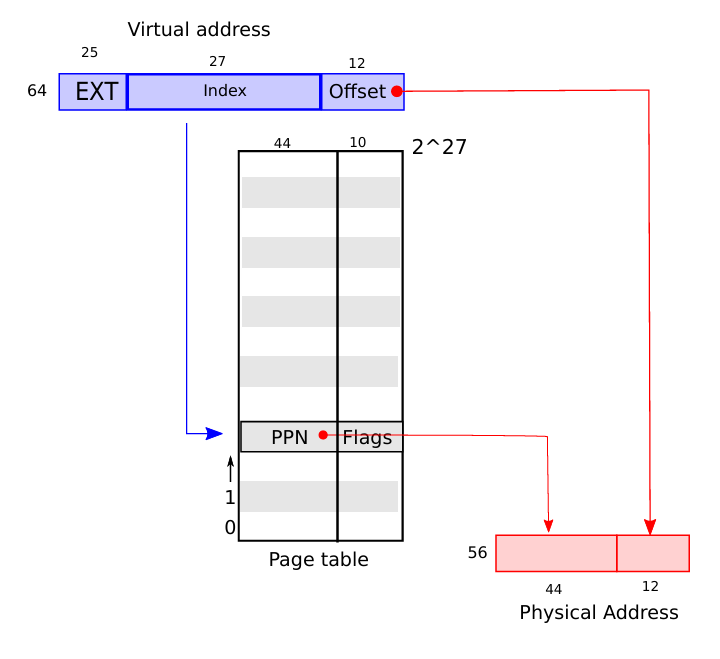
\includegraphics[width=0.7\textwidth]{RISC_simplified}
	\caption{RISC-V 虚拟和物理地址,具有简化的逻辑页表}
	\label{fig:RISC_simplified}
\end{figure}

\begin{figure}[!htb]
	\centering
	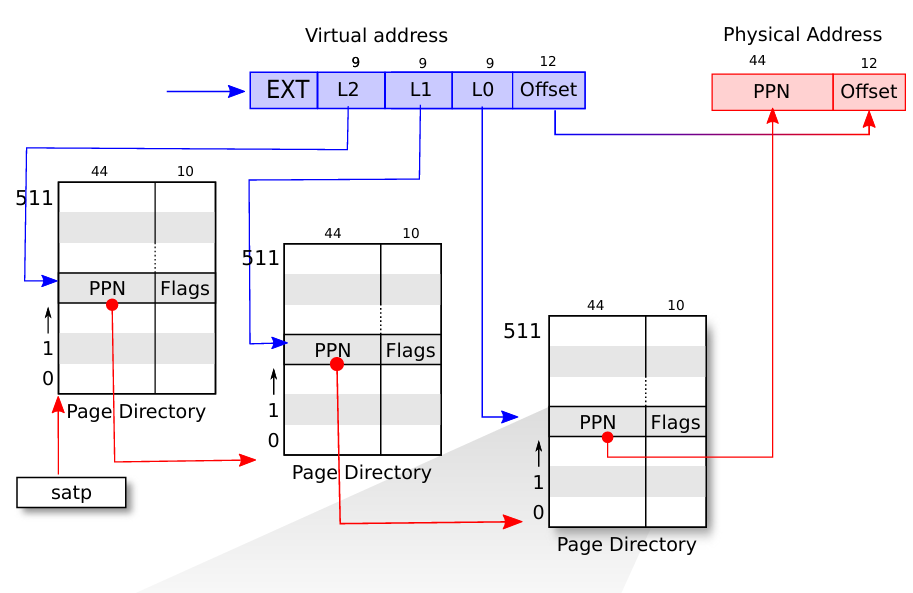
\includegraphics[width=0.8\textwidth]{RISC}
	\caption{RISC-V 地址转换的详细信息}
	\label{fig:RISC}
\end{figure}

\begin{table}[!hpt]
	\caption{PTE各个位的含义}
	\label{tab:pte-bits}
	\centering
	\begin{tabular}{@{}ccc@{}} \toprule
		\textbf{位数} & \textbf{名称} & \textbf{作用} \\ 
		\midrule
		0   & V  & 有效位(Valid) \\
		1   & R  & 读权限(Read) \\
		2   & W  & 写权限(Write) \\
		3   & X  & 执行权限(Execute) \\
		4   & U  & 用户态可访问(User) \\
		5   & G  & 全局映射(Global) \\
		6   & A  & 访问位(Accessed) \\
		7   & D  & 脏页位(Dirty) \\
		8-9   & 保留 & 未使用 \\
		10-53 & PPN & 物理页号(Physical Page Number) \\
		54-63 & 保留 & 未使用 \\
		\bottomrule
	\end{tabular}
\end{table}

\begin{figure}[!htb]
	\centering
	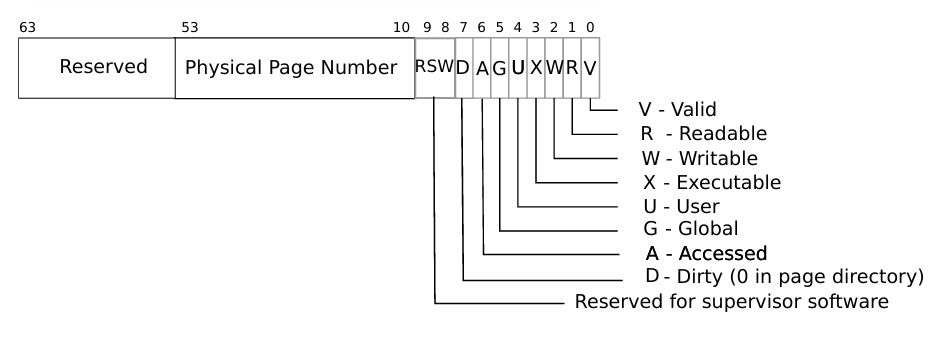
\includegraphics[width=0.8\textwidth]{PTE}
	\caption{PTE各个位的含义}
	\label{fig:PTE}
\end{figure}

\subsubsection{内核地址空间}

每个进程有一个页表,用于描述进程的用户地址空间,还有一个内核地址空间(所有进程共享这一个描述内核地址空间的页表)。为了让内核使用物理内存和硬件资源,内核需要按照一定的规则排布内核地址空间,以能够确定哪个虚拟地址对应自己需要的硬件资源地址。用户地址空间不需要也不能够知道这个规则,因为用户空间不允许直接访问这些硬件资源。

如\cref{fig:kernel_address_space} 所示,QEMU会模拟一个从0x80000000开始的RAM,一直到0x86400000。QEMU会将设备接口以控制寄存器的形式暴露给内核,这些控制寄存器在0x80000000以下。kernel对这些设备接口控制寄存器的访问是直接和这些设备而不是RAM进行交互的。用户地址的空间分配在free memory中。

\begin{figure}[!htb]
	\centering
	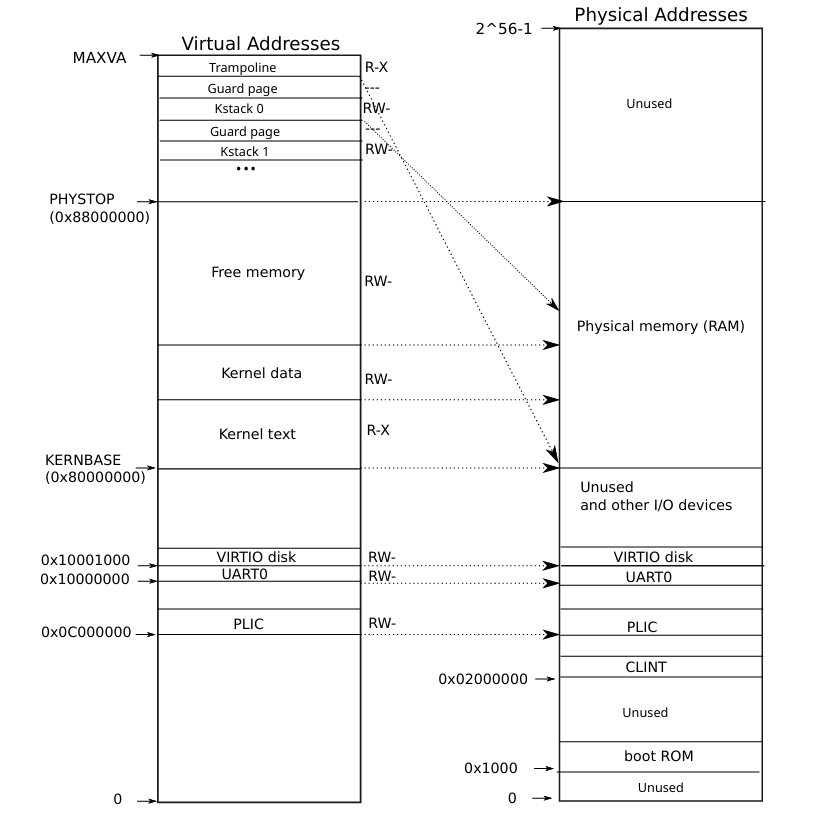
\includegraphics[width=0.8\textwidth]{kernel_address_space}
	\caption{xv6 的内核地址空间(左)和期望看到的RISC-V物理地址空间(右)}
	\label{fig:kernel_address_space}
\end{figure}

\subsubsection{进程地址空间}

每个进程有自己的用户空间下的虚拟地址,这些虚拟地址由每个进程自己的页表维护,用户空间下的虚拟地址从0到MAXVA。

\cref{fig:process_address_space} 是一个进程在刚刚被exec调用时的用户空间下的内存地址,stack只有一页,包含了 \texttt{exec}调用的命令的参数从而使 \texttt{main(argc, argv)} 可以被执行。stack下方是一个guard page来检测stack溢出,一旦溢出将会产生一个page fault exception

\cref{lst:relevant_variables} 展示了部分变量在xv6代码中的定义:
\begin{enumerate}
	\item MAXVA :表示用户空间可用的最大虚拟地址。RISC-V Sv39 虚拟地址空间为39位,分为三级页表,每级九位索引,页内偏移12位,但xv6为了避免高位符号扩展问题,实际只用到38位(最高位不用)。
	\item TRAMPOLINE :虚拟地址空间中最高的一页,所有进程的虚拟地址空间都把这一页映射到同一个物理页。其作用是存放trampoline.S中的汇编代码,用于用户态和内核态切换时保存/恢复上下文(trap/ret)。
	例如,用户进程发生系统调用或中断时,CPU会跳转到TRAMPOLINE页执行trap处理代码。
	\item TRAPFRAME : TRAMPOLINE 下方的一页,用于保存用户进程在陷入内核(trap)时的所有寄存器内容,包括PC、SP、通用寄存器等。
	\item USYSCALL : TRAPFRAME 再往下的一页,用于内核向用户空间传递只读信息(如pid等)。
\end{enumerate}

\begin{listing}[!htb]
	\begin{minted}{c}
#define PGSIZE 4096
#define MAXVA (1L << (9 + 9 + 9 + 12 - 1))
#define TRAMPOLINE (MAXVA - PGSIZE)
#define TRAPFRAME (TRAMPOLINE - PGSIZE)
#define USYSCALL (TRAPFRAME - PGSIZE)
	\end{minted}
	\caption{相关变量在xv6中的定义}\label{lst:relevant_variables}
\end{listing}

\begin{figure}[!htb]
	\centering
	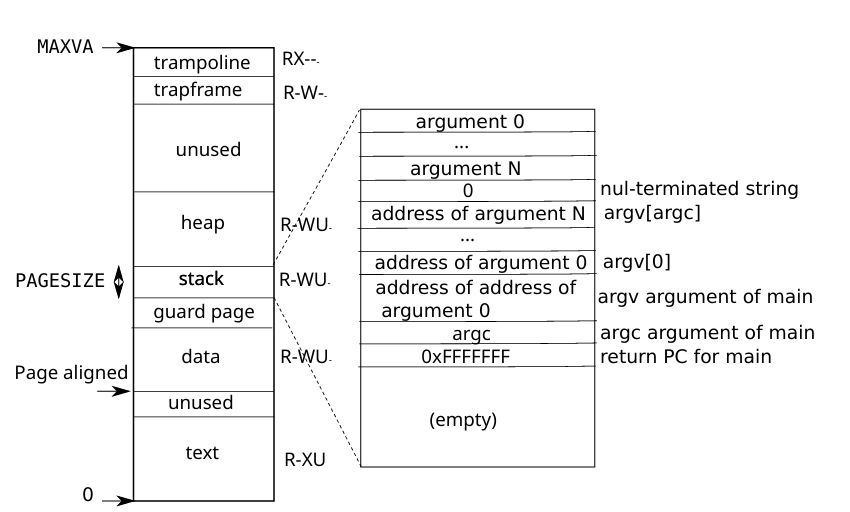
\includegraphics[width=0.8\textwidth]{process_address_space}
	\caption{进程的用户地址空间及其初始堆栈}
	\label{fig:process_address_space}
\end{figure}

\subsubsection{创建地址空间}

xv6中和页表相关的代码在 \texttt{kernel/vm.c} 中。最主要的结构体是 \texttt{pagetable\_t},这是一个指向页表的指针。\texttt{kvm} 开头的函数都是和kernel virtual address(内核虚拟地址)相关的,\texttt{uvm}开头的函数都是和user virtual address(用户虚拟地址)相关的,其他的函数可以用于这两者。

几个比较重要的函数:
\begin{enumerate}
	\item \texttt{walk}:给定一个虚拟地址和一个页表,返回一个PTE指针。
	\item \texttt{mappages}:给定一个页表、一个虚拟地址和物理地址,创建一个PTE以实现相应的映射。
	\item \texttt{kvminit}:用于创建kernel的页表,使用 \texttt{kvmmap} 来设置映射
	\item \texttt{kvminithart}:kernel的页表的物理地址写入CPU的寄存器 \texttt{satp} 中,CPU利用这个kernel页表翻译地址。
	\item \texttt{procinit}:(\texttt{kernel/proc.c})为每一个进程分配(kalloc)kstack。KSTACK会为每个进程生成一个虚拟地址(同时也预留了guard pages),\texttt{kvmmap}将这些虚拟地址对应的PTE映射到物理地址中,然后调用\texttt{kvminithart}来重新把kernel页表加载到\texttt{satp}中去。
\end{enumerate}

\subsection{实验步骤}

\subsubsection{实现加速系统调用}

实现步骤:
\begin{enumerate}
	\item 在 \texttt{kernel/memlayout.h} 中查看 \texttt{usyscall} 结构体的定义,如\cref{lst:usyscall} 所示。
	\item 在\texttt{proc}结构体中添加变量\texttt{usyscall},如\cref{lst:add_usyscall} 所示。
	\item 根据提示,在\texttt{proc\_pagetable} 中,参考前面的写法,添加对\texttt{p->usyscall} 的映射,如\cref{lst:proc_pagetable} 所示。
	\item 在 \texttt{allocproc} 中,添加对 \texttt{usyscall} 的分配和初始化,如\cref{lst:allocproc} 所示。
	\item 在 \texttt{freeproc} 中,添加对 \texttt{usyscall} 的释放,如\cref{lst:freeproc} 所示。
	\item 注意到 \texttt{freeproc} 中调用了 \texttt{proc\_freepagetable},需要对此添加对 \texttt{USYSCALL} 映射页的释放,如\cref{lst:proc_freepagetable} 所示。
	\item 测试加速系统调用,成功运行。如\cref{fig:test_pgtbltest} 所示。
\end{enumerate}

\begin{listing}[!htb]
	\begin{minted}{c}
struct usyscall{
    int pid; // Process ID
}
	\end{minted}
	\caption{usyscall结构体的定义}\label{lst:usyscall}
\end{listing}

\begin{listing}[!htb]
	\begin{minted}{c}
struct proc{
    ...
    struct usyscall *usyscall; // datapage for usyscall.S
}
	\end{minted}
	\caption{在proc结构体中添加变量usyscall}\label{lst:add_usyscall}
\end{listing}                                    

\begin{listing}[!htb]
	\begin{minted}{c}
pagetable_t
proc_pagetable(struct proc *p)
{
    ...
    // map the usyscall just below TRAPFRAME, for trapframe.S
    if(mappages(pagetable, USYSCALL, PGSIZE,
    (uint64)(p->usyscall), PTE_R | PTE_U) < 0){
        uvmunmap(pagetable, TRAPFRAME, 1, 0);
        uvmunmap(pagetable, TRAMPOLINE, 1, 0);
        uvmfree(pagetable, 0);
        return 0;
    }

    return pagetable;
}
	\end{minted}
	\caption{在proc\_pagetable中添加对p->usyscall的映射}\label{lst:proc_pagetable}
\end{listing}

值得注意的是,在\texttt{proc\_pagetable}中,对三个区域映射的PTE条件不一样,原因如下:
\begin{enumerate}
	\item trampoline 判断的权限是 PTE\_R 和 PTE\_X(可读+可执行),因为 trampoline 页存放的是trap/ret相关的汇编代码,只需要CPU执行和读取,不需要写入。不判断 PTE\_W 的原因是禁止写入,防止恶意或错误代码修改 trampoline 内容,保证内核和用户态切换的安全;不判断 PTE\_U 的原因是用户态不能直接访问,只能在陷入内核时由内核代码使用。
	
	\item trapframe 判断的权限是 PTE\_R 和 PTE\_W(可读+可写),因为 trapframe 用于保存用户进程的寄存器上下文,需要内核读写。不判断 PTE\_X 的原因是 trapframe 不是代码,不能被执行;不判断 PTE\_U 的原因是用户态不能访问,只能由内核读写,防止用户进程篡改自己的 trapframe,保证上下文切换的正确性和安全性。
	
	\item usyscall 判断的权限是 PTE\_R 和 PTE\_U(可读+可访问),因为usyscall 页用于内核向用户空间传递只读信息(如pid等),用户进程需要读取,但不能写入。不判断 PTE\_W 的原因是防止用户进程修改内核提供的信息;不判断 PTE\_X 的原因是 usyscall 不是代码,不能被执行。
	
\end{enumerate}

\begin{listing}[!htb]
	\begin{minted}{c}
static struct proc*
allocproc(void)
{
    struct proc *p;
    ...
    // Allocate a usyscall page.
    if((p->usyscall = (struct usyscall *)kalloc()) == 0){
        printf("allocproc: kalloc for usyscall failed!\n");
        freeproc(p);
        release(&p->lock);
        return 0;
    }
    p->usyscall->pid = p->pid;
    ...
}
	\end{minted}
	\caption{在allocproc中添加对usyscall的分配}\label{lst:allocproc}
\end{listing}

\begin{listing}[!htb]
	\begin{minted}{c}
static void
freeproc(struct proc *p)
{
    if(p->trapframe)
    kfree((void*)p->trapframe);
    p->trapframe = 0;
    if(p->usyscall)
        kfree((void*)p->usyscall);
    p->usyscall = 0;
    ...
}
	\end{minted}
	\caption{在freeproc中添加对usyscall的释放}\label{lst:freeproc}
\end{listing}

\begin{listing}[!htb]
	\begin{minted}{c}
void
proc_freepagetable(pagetable_t pagetable, uint64 sz)
{
    uvmunmap(pagetable, USYSCALL, 1, 0);
    ...
}
	\end{minted}
	\caption{在proc\_freepagetable增加对USYSCALL映射页的释放}\label{lst:proc_freepagetable}
\end{listing}

\begin{figure}[!htb]
	\centering
	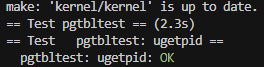
\includegraphics[width=0.4\textwidth]{test_pgtbltest}
	\caption{测试加速系统调用}
	\label{fig:test_pgtbltest}
\end{figure}

\subsubsection{实现打印页表}

\begin{enumerate}
	\item 在\texttt{kernel/vm.c}中创建\texttt{vmprint}函数,参数为\texttt{pagetable\_t },并在\texttt{exec}中调用,如\cref{lst:call_vmprint} 所示。
	\item 根据提示,阅读\cref{lst:freewalk},该函数通过遍历和递归页表来释放页表页面,\texttt{pte} 为页表项,用于描述虚拟地址到物理地址的映射关系,如果 \texttt{(pte \& PTE\_V) \&\& (pte \& (PTE\_R|PTE\_W|PTE\_X)) == 0}(PTE有效但是没有读/写/执行权限),说明该页表项指向下一级页表;如果 \texttt{(pte \& PTE\_V) != 0}(页表有效),说明该页表是叶子节点,实际映射到物理页。
	\item 仿照 \texttt{freewalk} 的结构,完成 \texttt{vmprintdfs} 函数,通过深度优先打印页表项,使用 \texttt{\%p} 打印十六进制PTE和地址,使用\texttt{PTE2PA} 获取从PTE中提取出的物理地址,如\cref{lst:vmprint} 所示。
	\item 测试打印页表,成功运行。如\cref{fig:test_pte_printout} 所示。
\end{enumerate}

\begin{listing}[!htb]
	\begin{minted}{c}
int exec(char *path,char **argv){
    ...
    struct proc *p = myproc();
    ...
    p = myproc();
    ...
    if(p->pid==1){
        vmprint(p->pagetable);
    }
    return args
    ...
}
	\end{minted}
	\caption{在exec中调用vmprint}\label{lst:call_vmprint}
\end{listing}

\begin{listing}[!htb]
	\begin{minted}{c}
void
freewalk(pagetable_t pagetable)
{
    // there are 2^9 = 512 PTEs in a page table.
    for(int i = 0; i < 512; i++){
    pte_t pte = pagetable[i];
        if((pte & PTE_V) && (pte & (PTE_R|PTE_W|PTE_X)) == 0){
            // this PTE points to a lower-level page table.
            uint64 child = PTE2PA(pte);
            freewalk((pagetable_t)child);
            pagetable[i] = 0;
        } else if(pte & PTE_V){
            panic("freewalk: leaf");
        }
    }
    kfree((void*)pagetable);
}
	\end{minted}
	\caption{freewalk函数的实现}\label{lst:freewalk}
\end{listing}

\begin{listing}[!htb]
	\begin{minted}{c}
void vmprintdfs(pagetable_t pagetable,int level){
    for(int i = 0;i < 512;i++){
        pte_t pte = pagetable[i];
         
        if((pte & PTE_V) && (pte & (PTE_R|PTE_W|PTE_X)) == 0){
            // 有效但没有R/W/X权限,说明指向下一级页表
            uint64 child = PTE2PA(pte);
            for(int j = 0;j <= level ; j++){
                printf(" ..");
            }
            printf("\%d: pte \%p pa \%p\n",i,pte,child);

            vmprintdfs((pagetable_t)child,level+1);
        }
        else if(pte & PTE_V){ // 叶子节点
            uint64 child = PTE2PA(pte);
            printf(".. .. ..\%d: pte \%p pa \%p\n",i,pte,child);
        }
    }
}

void vmprint(pagetable_t pagetable){
    printf("page table \%p\n",pagetable);
    vmprintdfs(pagetable,0);
}
	\end{minted}
	\caption{vmprint函数的实现}\label{lst:vmprint}
\end{listing}

\begin{figure}[!htb]
	\centering
	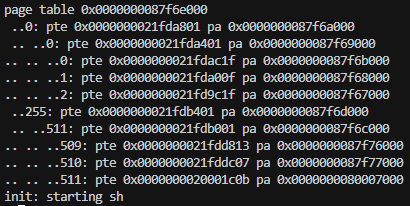
\includegraphics[width=0.6\textwidth]{test_pte_printout}
	\caption{测试打印页表}
	\label{fig:test_pte_printout}
\end{figure}

\subsubsection{实现检测哪些页面已被访问}

\begin{enumerate}
	\item 在 kernel/sysproc.c 中实现 \texttt{sys\_pgaccess(void)} ,该函数和 \texttt{pgaccess()} 一样,接受三个参数(用户页面的起始虚拟地址,待检查的页面数量,指向缓冲区的用户地址),并将结果存储到一个bitmask。
	\item bitmask 是一个32位的整数,用于记录32个页面的访问状态,第i位代表第i个页面是否被访问,使用位掩码能够快速、方便地读取、改变多个页面的访问状态。
	\item 函数 \texttt{argaddr(int n, uint64 *ip)} 和 \texttt{argaddr(int n, int *ip)} 的作用是解析第n个参数,并作为地址指针/int类型返回。使用它们来解析参数,另外还需要检查页面数量\texttt{len} 的合法性。
	\item 在 kernel/riscv.h 中定义 PTE\_A ,如\cref{lst:define_PTE_A} 所示。
	\item 设置一个临时缓冲区 \texttt{res},等到将其所有位都填充后,再通过 \texttt{copyout()} 函数将数据复制到用户。函数\texttt{int copyout(pagetable\_t pagetable, uint64 dstva, char *src, uint64 len)} 用于把内核空间的数据复制到用户空间。常用于系统调用返回数据给用户进程。其中,\texttt{pagetable}是目标进程的页表;\texttt{dstva}是用户空间的目标虚拟地址;\texttt{src}是内核空间的源数据指针;\texttt{len}是要复制的字节数,函数的具体实现如\cref{lst:copyout} 所示。
	\item 遍历页表的每一页,对于每一页,使用函数 \texttt{vmpgaccess()} 获取该页是否被访问,将该页的访问结果返回到 \texttt{abit},并通过位运算 \texttt{res = res | abit << i} 存储到临时缓冲区中。
    \item 函数\texttt{int vmpgaccess(pagetable\_t pagetable,uint64 va)} 接收页表和64位虚拟地址,并使用函数 \texttt{pte\_t *pte = walk(pagetable,va,0)}获取当前页表项 。函数\texttt{pte\_t *walk(pagetable\_t pagetable, uint64 va, int alloc)}从多级页表中查找某个虚拟地址对应的页表项(PTE)。其中\texttt{pagetable}是顶级页表的指针(当前进程的页表);\texttt{va}是要查找的虚拟地址;\texttt{alloc}表示是否在缺页时分配中间页表(1为分配,0为不分配),函数的具体实现如\cref{lst:walk} 所示。
    \item 获取页表项 \texttt{pte} 后,检查其 PTE\_A 位是否为1,判断语句为 \texttt{(*pte \& PTE\_A) != 0},若满足条件,则通过 \texttt{ *pte = *pte \& (~PTE\_A);} 将 \texttt{pte} 的 PTE\_A 位置零,并返回1表示 PTE\_A 位被访问过。
    \item 函数 \texttt{int vmpgaccess(pagetable\_t pagetable,uint64 va)} 和 函数 \texttt{sys\_pgaccess(void)} 的具体实现如\cref{lst:vmpgaccess} 和 \cref{lst:sys_pgaccess} 所示。
	\item 测试检测哪些页面已被访问,成功运行。如\cref{fig:test_pgacess} 所示。
\end{enumerate}

\begin{listing}[!htb]
	\begin{minted}{c}
#define PTE_V (1L << 0) // valid
#define PTE_R (1L << 1) // read
#define PTE_W (1L << 2) // write
#define PTE_X (1L << 3) // execute
#define PTE_U (1L << 4) // 1 -> user can access
#define PTE_A (1L << 6) // accessed
	\end{minted}
	\caption{PTE的相关定义}\label{lst:define_PTE_A}
\end{listing}

\begin{listing}[!htb]
	\begin{minted}{c}
int
copyout(pagetable_t pagetable, uint64 dstva, char *src, uint64 len)
{
    uint64 n, va0, pa0;

    while(len > 0){
        va0 = PGROUNDDOWN(dstva);
        pa0 = walkaddr(pagetable, va0);
        if(pa0 == 0)
            return -1;
        n = PGSIZE - (dstva - va0);
        if(n > len)
            n = len;
        memmove((void *)(pa0 + (dstva - va0)), src, n);

        len -= n;
        src += n;
        dstva = va0 + PGSIZE;
    }
    return 0;
}
	\end{minted}
	\caption{copyout函数的实现}\label{lst:copyout}
\end{listing}

\begin{listing}[!htb]
	\begin{minted}{c}
pte_t *
walk(pagetable_t pagetable, uint64 va, int alloc)
{
    if(va >= MAXVA)
    panic("walk");

    for(int level = 2; level > 0; level--) {
        pte_t *pte = &pagetable[PX(level, va)];
        if(*pte & PTE_V) {
            pagetable = (pagetable_t)PTE2PA(*pte);
        } else {
            if(!alloc || (pagetable = (pde_t*)kalloc()) == 0)
                return 0;
            memset(pagetable, 0, PGSIZE);
            *pte = PA2PTE(pagetable) | PTE_V;
        }
    }
    return &pagetable[PX(0, va)];
}
	\end{minted}
	\caption{walk函数的实现}\label{lst:walk}
\end{listing}

\begin{listing}[!htb]
	\begin{minted}{c}
int vmpgaccess(pagetable_t pagetable,uint64 va)
{
    pte_t *pte;

    if(va >= MAXVA)
    return 0;

    pte = walk(pagetable, va, 0);

    if(pte == 0)
        return 0;
    if((*pte & PTE_A) != 0){
        *pte = *pte & (~PTE_A);
        return 1;
    }
    
    return 0;
}
	\end{minted}
	\caption{vmpgaccess函数的实现}\label{lst:vmpgaccess}
\end{listing}

\begin{listing}[!htb]
	\begin{minted}{c}
sys_pgaccess(void)
{
    uint64 addr;  
    int len;
    int bitmask;
    
    if(argaddr(0, &addr) < 0)
        return -1;
    if(argint(1, &len) < 0)
        return -1;
    if(argint(2, &bitmask) < 0)
        return -1;
    if(len > 32 || len < 0)
        return -1;

    int res = 0;

    struct proc *p = myproc();
    for(int i = 0;i < len ;i++){
        uint64 va = addr + i * PGSIZE;
        int abit = vmpgaccess(p->pagetable,va);
        res = res | abit << i;
    }

    if(copyout(p->pagetable, bitmask, (char *)&res, sizeof(res)) < 0)
        return -1; 

    return 0;
}
	\end{minted}
	\caption{sys\_pgaccess函数的实现}\label{lst:sys_pgaccess}
\end{listing}

\begin{figure}[!htb]
	\centering
	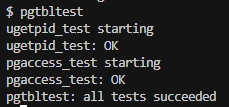
\includegraphics[width=0.5\textwidth]{test_pgacess}
	\caption{测试检测哪些页面已被访问}
	\label{fig:test_pgacess}
\end{figure}

\subsubsection{综合测试}

在xv6-labs-2021目录下创建一个time.txt文件,记录我完成该lab花费的时间,再创建一个answers-pgtbl.txt 文件,记录我对实验中问答题的答案。使用 \texttt{make grade} 对lab3进行综合测试,测试通过。

\begin{figure}[!htb]
	\centering
	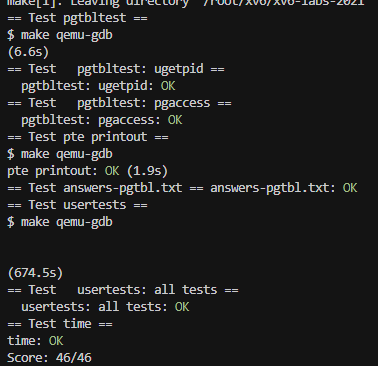
\includegraphics[width=0.5\textwidth]{test_lab3}
	\caption{测试lab3}
	\label{fig:test_lab3}
\end{figure}

\subsection{实验小结}

这个实验是我目前花费时间最多的实验。本次实验通过对xv6操作系统页表机制的深入探索和实际编程实现,使我对RISC-V多级页表结构、虚拟地址到物理地址的映射原理有了更为直观和深刻的理解。在动手实现用户空间与内核空间共享只读数据页、递归打印页表结构以及检测页面访问状态等功能的过程中,我不仅掌握了页表项各个位的具体作用和内核与用户空间数据交互的方法,还体会到操作系统在内存管理和安全性设计上的细致考量。实验过程中遇到的各种问题也锻炼了我的调试和独立解决问题的能力。总体而言,这次实验极大地提升了我对操作系统虚拟内存管理机制的理解和实际开发能力,为后续深入学习操作系统相关内容打下了坚实基础。
